\documentclass[8pt,c,compress,UTF8]{ctexbeamer}
\usepackage{ctex}
\usepackage{caption}
\usepackage{graphicx}
\usepackage{amsmath}
\usepackage{listings}

\usetheme{AnnArbor}
\usecolortheme{dolphin}
\usefonttheme{serif}

\title{Julia 集的分析和探索}
\author{杨钧尹}
\institute{浙江大学 数学科学学院}

\begin{document}

\thispagestyle{empty}   %使封面没有导航条
\maketitle

\section{引言}

% Page2
\begin{frame}
\frametitle{从分形理论说起}
\centering
Julia 集是一种在复平面上非发散点形成的分形点的集合。
\begin{figure}[htbp]
\centering
\begin{minipage}{0.33\linewidth}
\centering
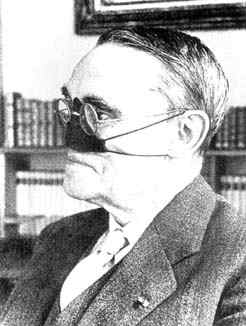
\includegraphics[width = 2.2cm]{./images/julia.jpg}
\caption*{\small Gaston Maurice Julia}
\end{minipage}\hfill
\begin{minipage}{0.33\linewidth}
\centering
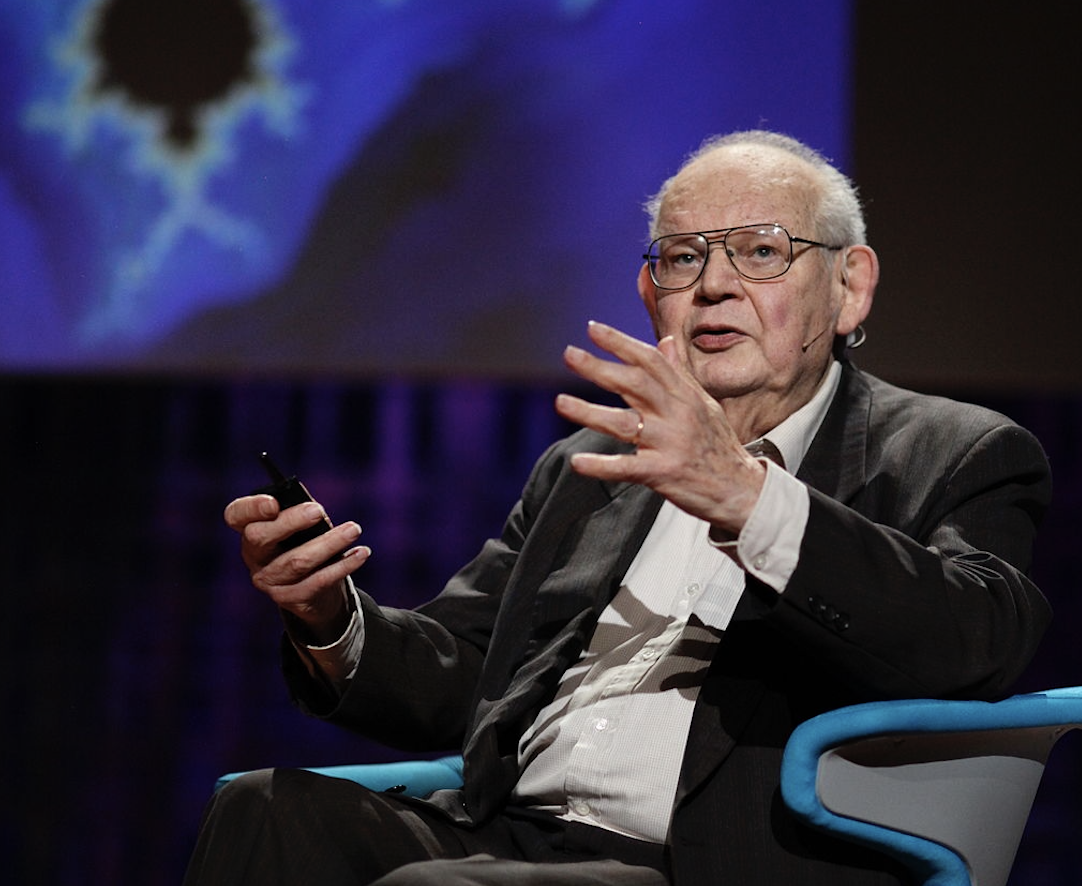
\includegraphics[width = 3.5cm]{./images/mandelbort.png}
\caption*{\small Benoit B. Mandelbrot}
\end{minipage}\hfill
\begin{minipage}{0.33\linewidth}
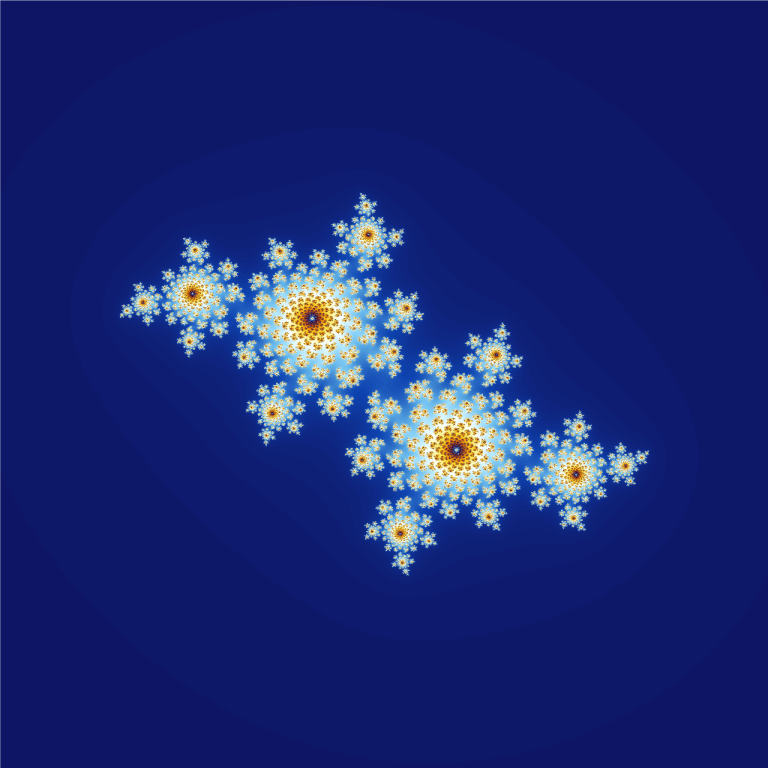
\includegraphics[width = 2.85cm]{./images/julia_set_example.png}
\centering
\caption*{\small $c=−0.4+0.6i$的例子}
\end{minipage}
\end{figure}
\begin{description}
\item[自相似性]整体与局部以某种方式相似。
\item[分形]具有自相似性的形体。\\Fractal:具有不规则、支离破碎等意义。
\end{description}
\end{frame}

\section{理论}

% page3
\subsection{定义}
\begin{frame} 
\frametitle{复二次多项式定义}
迭代公式:
$$f_c(z)=z^2+c$$
\begin{block}{Julia 集}
对于固定的复数c,取某一z值(如$z=z_0$),可以得到序列
$$(z_0,f_c(z_0),f_c(f_c(z_0)),f_c(f_c(f_c(z_0)))\cdots)$$
这一序列可能发散于无穷大或始终处于某一范围之内并收敛于某一值。我们将\alert{使其不扩散的z值的集合}称为 Julia 集。
\end{block}
\begin{block}{Mandelbrot 集}
而若从$z=0$开始对$f_c(z)$进行$z_{n+1}=z^2_n+c,n=0,1,2,\cdots$迭代,
可以得到序列
$$(0,f_c(0),f_c(f_c(0)),f_c(f_c(f_c(0)))\cdots)$$
构建出\alert{使序列不延伸至无限大的所有复数$c$的集合},称为 Mandelbrot 集。
\end{block}
Julia 集是在固定$c$的情形下计算发散的$z$的值,决定图案形状的因素有且仅有$c$。

倘若将所有$c$情形的 Julia 集刻画于同一复域平面上,则可以得到 Mandelbrot 集。
\end{frame}

% page4
\subsection{特性}
\begin{frame} 
\frametitle{基本定义}
\begin{itemize}
    \item 迭代方式决定了 Julia 集是无限的。
    \item \alert{【定理】Fundamental Dichotomy Theorem}

    一个 Julia 集或者是完全连通的,任意两点间都有一条通路;或者是完全不连通的,整个图形全是一个个孤立的点。
    \item Julia 集和 Mandelbrot 集都具有自相似性。
\end{itemize}
\begin{block}{结论}
连通的 Julia 集所对应的参数就是 Mandelbrot 集中的点
Mandelbrot 集则可以视作所有二次 Julia 集的缩略图。
他们在相同$c$的情形下存在结构与形态上的紧密联系。
\end{block}
\end{frame}

\section{算法}

% page5
\subsection{基本思路}
\begin{frame} 
\frametitle{设计算法的步骤和思路} 
我们通常假设$|c|<2$,那么经过$k$次迭代后,倘若$|z|>2$,这意味着
$|z^2|=|z|^2>2\cdot|z|$,显然,$|z|$自此随着迭代越来越大,即该点发散。反之,这样的点可以构成
的模抵消到原来的水平。因此,在迭代运算过程中,一旦某一步结果的模大于 2 了,可以断定它必将发散到无穷。
{\noindent}  \rule[-10pt]{12.2cm}{0.05em}\\
\begin{columns}
\column{0.5\textwidth}
但在实际计算中,我们无法找出所有的收敛点;
采取有限逼近的方法寻找所有模不大于 2 的点集;
转化为对平面网格上所有点遍历的一般算法:
\begin{itemize}
    \item 收敛判定,确定是否填色。
    \item 填充颜色,输出为bmp图像。
\end{itemize}
\column{0.5\textwidth}
\begin{itemize}
    \item 迭代次数$N$:控制最大迭代次数,理论上数值越大,图像越精细。
    \item 图像中心坐标$ox,oy$:控制生成图像在画布上的中心位置。
    \item 图像半径尺寸$Dimension$:实现缩放效果。
    \item Julia 迭代参数$c$的实部和虚部:控制该参数,改变生成图像形态。
\end{itemize}
\end{columns}
\end{frame}

% page6
\subsection{伪代码}
\begin{frame}[fragile]
\frametitle{设计算法的步骤和思路}
\begin{block}{算法伪代码:}
\begin{lstlisting}
    R = escape radius  # R > 0 && R^2 - R >= sqrt(cx^2 + cy^2)
    For Each Pixel(x,y) on the screen:
        zx = scaled x coordinate of pixel;
        zy = scaled y coordinate of pixel;
        iteration = 0;
        max_iteration = 1000;
        while (zx * zx + zy * zy < R^2  &&  iteration < max_iteration)
            xtemp = zx * zx - zy * zy;
            zy = 2 * zx * zy  + cy;
            zx = xtemp + cx;
            iteration = iteration + 1;
        if (iteration == max_iteration): let the pixel be black;
        else: return iteration;
    Finish drawing pixels, output the bmp file.
\end{lstlisting}
\end{block}
\end{frame}

\section{算例分析}
% page7
\subsection{图像分析}
\begin{frame} 
\subsection{图像分析}
\begin{figure}[htbp]
\centering
\begin{minipage}{0.33\linewidth}
\centering
\includegraphics[width = 3.5cm]{./images/julia2-1.bmp}
\caption{100,0,0,2,-0.4,0.6}
\label{fig2-1}
\end{minipage}\hfill
\begin{minipage}{0.33\linewidth}
\centering
\includegraphics[width = 3.5cm]{./images/julia2-2.bmp}
\caption{100,0,0,2,-0.6,-0.4}
\label{fig2-2}
\end{minipage}\hfill
\begin{minipage}{0.33\linewidth}
\centering
\includegraphics[width = 3.5cm]{./images/julia2-3.bmp}
\caption{100,0,0,2,-0.8,0.16}
\label{fig2-3}
\end{minipage}
\end{figure}

\end{frame}

% page8
\subsection{算法检验}
\begin{frame} 
\frametitle{算法检验}

\begin{figure}[htbp]
\centering
\begin{minipage}{0.33\linewidth}
\centering
\includegraphics[width = 3.5cm]{./images/julia3-1.bmp}
\caption{40,0,0,2,-0.4,0.6}
\label{fig3-1}
\end{minipage}\hfill
\begin{minipage}{0.33\linewidth}
\centering
\includegraphics[width = 3.5cm]{./images/julia3-2.bmp}
\caption{100,0,0,1,-0.6,-0.4}
\label{fig3-2}
\end{minipage}\hfill
\begin{minipage}{0.33\linewidth}
\centering
\includegraphics[width = 3.5cm]{./images/julia3-3.bmp}
\caption{100,0.6,0.5,2,-0.8,0.16}
\label{fig3-3}
\end{minipage}
\end{figure}

\end{frame}

% page9
\subsection{特性比较}
\begin{frame} 
\frametitle{特性比较}

\begin{figure}[htb]
\centering
\begin{minipage}{0.45\linewidth}
\centering
\includegraphics[width = 3.5cm]{./images/julia4-1.bmp}
\caption*{Julia,100,0,0,3,0.25,0}
\label{fig4-1}
\end{minipage}\hfill
\begin{minipage}{0.45\linewidth}
\centering
\includegraphics[width = 3.5cm]{./images/mandel4-3.bmp}
\caption*{Mandelbrot,100,0.4,0,1}
\label{fig4-2}
\end{minipage}
\end{figure}

\end{frame}

\section{结论}
% page10
\begin{frame} 
\frametitle{总结}
\begin{block}{}
        这是一个区块
\end{block}
\begin{description}
\item[First Item] Description of first item
\item[Second Item] Description of second item
\item[Third Item] Description of third item
\item[Forth Item] Description of forth item
\end{description}
\end{frame}

\end{document}